\documentclass{article}
\usepackage{amsmath}
\usepackage{amssymb}
\usepackage{graphicx}
\usepackage{hyperref}
\usepackage[version=4]{mhchem}


\begin{document}
\section*{Problem}
\(A B C D\) is a quadrilateral with \(A D / / B C\). Draw \(A G \perp A B\) to meet \(D C\) at \(F\) and the extension of \(B C\) at \(G\). Points \(E\) is the midpoint of sides \(B G\). Find the length \(A E\) if \(A D=\) 2.7, \(A F=4\), and \(A B=6\).\\
\centering
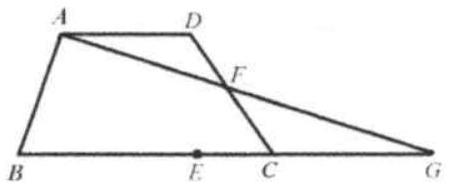
\includegraphics[width=\textwidth]{images/016(1).jpg}

\section*{Solution}
\(m^{2}\).\\
Draw the perpendicular line \(A D\) and \(A D \perp B C\) at \(D\).

Since \(A B=A C\), and \(A D \perp B C, B D=C D\).\\
\(P A^{2}+P B \times P C\)\\
\(=P A^{2}+(B D-P D) \times(C D+P D)\)\\
\(=P A^{2}+(C D-P D) \times(C D+P D)\)\\
\centering
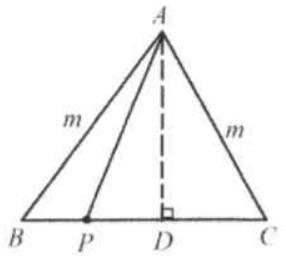
\includegraphics[width=\textwidth]{images/094.jpg}\\
\(=P A^{2}+C D^{2}-P D^{2}\)\\
\(=P A^{2}-P D^{2}+C D^{2}\)\\
\(=A D^{2}+C D^{2}=m^{2}\).

\end{document}
